\documentclass[tikz,border=10pt]{standalone}
% Quadrilateral ABCD with diagonals AD and BC; no right-angle marks, P unlabeled.
\begin{document}
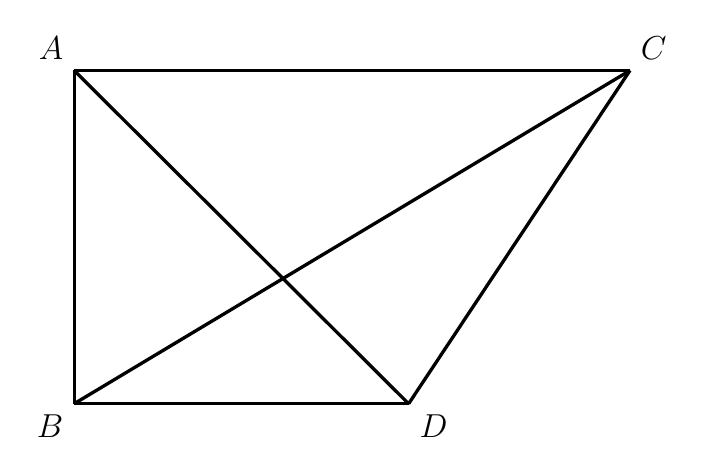
\begin{tikzpicture}[line width=1.2pt, line join=round]
  % Vertices in cm (scale s = 0.014953 cm/px, y flipped)
  \coordinate (A) at (1.0317,-0.6878);
  \coordinate (B) at (1.0317,-4.9201);
  \coordinate (C) at (8.0906,-0.6878);
  \coordinate (D) at (5.2793,-4.9201);
  % Interior crossing point of diagonals (not labelled)
  \coordinate (P) at (3.6850,-3.3260);

  % Edges
  \draw (A) -- (C);
  \draw (A) -- (B);
  \draw (B) -- (D);
  \draw (C) -- (D);
  \draw (A) -- (D);
  \draw (B) -- (C);

  % Labels
  \node[above left,  font=\fontsize{12}{14.4}\selectfont] at (A) {$A$};
  \node[above right, font=\fontsize{12}{14.4}\selectfont] at (C) {$C$};
  \node[below left,  font=\fontsize{12}{14.4}\selectfont] at (B) {$B$};
  \node[below right, font=\fontsize{12}{14.4}\selectfont] at (D) {$D$};
\end{tikzpicture}
\end{document}